\documentclass[a4paper]{article}
\usepackage[UTF8]{ctex}
\usepackage{ulem}\usepackage{ulem}
\usepackage{fancyhdr}
\usepackage{geometry}
\usepackage{listings}
\usepackage{amssymb}
\usepackage{hyperref}
\usepackage{xeCJKfntef}
\usepackage{array}
\usepackage{tikz}
\usepackage{booktabs}
\usepackage{multirow}
\usepackage{yhmath}
\usepackage{amsmath}
\usepackage{graphicx}  %%  图片包
\usepackage{subfig}    %% 子图包
% \usepackage{ctex}      
\usepackage{float}     %% 浮动个数
\usepackage{amsthm}
% \usepackage[usenames,dvipsnames]{xcolor}
\newtheorem{theorem}{定理}[section]
\newtheorem{lemma}{引理}[section]
\newtheorem{corollary}{推论}[section]
\newtheorem{exam}{例}[subsection]
\newtheorem{definition}{定义}[section]
\newtheorem{axiom}{公理}[section]
\usetikzlibrary{angles, calc}
\usetikzlibrary{intersections, through}

\tikzset{
  dot/.style={
    circle, fill=black, inner sep=1pt, outer sep=0pt
  },
  dot label/.style={
    circle, inner sep=0pt, outer sep=1pt
  },
  % style for every pics named "right angle"
  pics/right angle/.append style={
    /tikz/draw, /tikz/angle radius=5pt
  }
}

\title{基础数学知识}
\author{屈泰瑞 XiaoQuQu}
\date{\today}

% \geometry{papersize=A4}
\geometry{left=1cm,right=1cm,top=2cm,bottom=2cm}

\pagestyle{fancy}

\lhead{\bf 基础数学知识}
\chead{}
\rhead{屈泰瑞}
\lfoot{}
\cfoot{\thepage}
\renewcommand{\headrulewidth}{0.4pt}
\renewcommand{\footrulewidth}{0.4pt}

\begin{document}

\maketitle

\newpage

\section{数论基础}

\subsection{数域}

\begin{definition}
    对于一个数的集合 $F$,如果 $\forall a,b\in F$,都有 $a+b,a-b,a\times b,\frac
        {a}{b}(b\ne 0) \in F$,那么 $F$ 就称为一个数域.
\end{definition}

几个常见的数域都有自己的记号,如有理数域 $Q$,实数域 $R$,复数域 $C$. 但注意,自然数的集合 $N$ 不是一个域. 如果
一个数域 $F$ 里的每一个数都在另一个数域 $P$ 里,那么称 $F$ 是 $P$ 的一个子域.

\begin{theorem}
    有理数域 $Q$ 是最小的数域.
\end{theorem}

\begin{proof}
    根据数域的定义,有 $0,1\in F$.

    于是,有 $1\in F, 1+1\in F,\cdots, x\in F(x\in Z^+)$. 其中,$Z^+$ 为正整数集合.

    同样的,有 $-1\in F,-1-1\in F,\cdots, x\in F(x\in Z)$. 其中,$Z$ 为整数集合.

    根据除法的封闭性,有 $Q\subseteq F$.
\end{proof}

\begin{theorem}
    若 $F_1,F_2$ 为数域,则 $F_1 \cap F_2$ 也为数域.
\end{theorem}

证明显然.

\subsection{整除}

\begin{definition}
    对于两个整数 $a,b$,若 $a\ne 0$ 且存在 $c \in Z$ 使得 $b=ca$,那么我们称 $b$ 可被
    $a$ 整除,记作 $a\mid b$,否之,记作 $a \nmid b$.
\end{definition}

若对于两个整数 $a,b$,有 $a\mid b$,我们称 $a$ 为 $b$ 的因数,$b$ 为 $a$ 的倍数.

\subsection{最小公倍数、最大公因数}

\begin{definition}
    对于给定的 $a,b$,记最大使得 $x \mid a,x \mid b$ 的 $x\in Z$ 为 $a,b$ 的最大公因数
    ,记作 $\gcd(a,b)$. 记最小使得 $a\mid x,b\mid x$ 的 $x \in Z$ 为 $a,b$ 的最小
    公因数,记作 $\operatorname{lcm}(a,b)$.
\end{definition}

\begin{theorem}
    对于给定的 $a,b$,$\gcd(a,b)\times \operatorname{lcm}(a,b)=a\times b$.
\end{theorem}

\begin{proof}
    设 $x=\gcd(a,b),y=\operatornamewithlimits{lcm}(a,b)$.

    则 $a=m\times x,b=n\times x$,$n$ 与 $m$ 应为互质关系.

    故 $y=m\times n\times x$.

    等式两边同乘 $x$,即 $x\times y=m\times n\times x^2=a\times b$. 得证.
\end{proof}

若两个整数 $a,b$ 有 $\gcd(a,b)=1$,那么我们称 $a,b$ \textbf{互素}. 如,$2,3$ 就是
一对互素的数,$2,4$ 不是一对互素的数,因为 $\gcd(2,4)=2\ne 1$.

显然,质数与任一非自身倍数的数都互素.

\subsection{同余}

\begin{definition}
    若有 $a\in Z,b\in Z$ 使得 $a=xm+r,b=ym+r$,我们就称 $a,b$ 在模 $m$ 意义下同余,
    记作 $a\equiv b \pmod m$.
\end{definition}

同余有非常多的性质,简单列举几条容易被发现的性质.

\begin{itemize}
    \item 自反性,$a\equiv a\pmod m$.
    \item 传递性,若 $a\equiv b\pmod m,b\equiv c \pmod m$,那么
          $a\equiv c\pmod m$.
\end{itemize}

\begin{theorem}
    设 $a,b \in Z, k,n\in N^*$,若 $a\equiv b \pmod m$,那么
    $ak\equiv bk \pmod {mk}$.
\end{theorem}

\begin{proof}
    设 $a=xm+r,b=ym+r$.

    那么有
    \begin{equation*}
        \begin{split}
            ak-bk&\equiv (xm+r)k-(ym+r)k\pmod {mk}\\
            &\equiv xmk+rk-ymk-rk\\
            &\equiv (x-y)mk\\
            &\equiv 0
        \end{split}
    \end{equation*}

    因为有 $ak-bk\equiv 0 \pmod {mk}$,所以有 $ak \equiv bk \pmod {mk}$.
\end{proof}

同余还有一个很重要的性质.

\begin{theorem}
    当 $a\equiv b \pmod m$ 时,设 $x\in Z$,以下等式均成立.

    \begin{itemize}
        \item $a+x \equiv b+x \pmod m$.
        \item $a-x \equiv b-x \pmod m$.
        \item $a\times x \equiv b\times x \pmod m$.
    \end{itemize}
\end{theorem}

\begin{proof}
    这里仅证明 $a\times x \equiv b\times x \pmod m$,其他情况同理.

    设 $a=qm+r,b=pm+r$,那么我们有

    \begin{equation*}
        \begin{split}
            ax-bx &\equiv (qm+r)x-(pm+r)x\pmod m\\
            &\equiv qmx-pmx\\
            &\equiv 0
        \end{split}
    \end{equation*}

    所以有 $a\times x \equiv b\times x \pmod m$.
\end{proof}

注意,若有 $a\equiv b\pmod m$,不一定有 $\frac{a}{c}\equiv \frac{b}{c}\pmod m$. 事实上,该式大部分时间不成立,
能使 $ac^{-1}\equiv bc^{-1}\pmod m$ 的 $c^{-1}$ 称为 $c$ 在模 $m$ 意义下的乘法逆元.

\begin{lemma}
    若 $\gcd(a,b)=1$,必然不存在 $c\in [0,b-1]$ 使得 $ac\equiv 0\pmod b$.
\end{lemma}

\begin{proof}
    反证法. 设 $b\mid ac$,因为 $\gcd(a,b)=1$,所以 $b\mid c$. 但 $c<b$,与 $b\mid c$ 矛盾. 故不存在 $c$ 使得
    $b \mid ac$.
\end{proof}

\begin{lemma}
    当 $\gcd(a,m)=1$ 时,必定唯一存在 $c$ 使得 $ac\equiv 1\pmod m$.
\end{lemma}

\begin{proof}
    设 $S=\{0,1,\cdots,m-1\},A=\{0\times a \bmod m,1\times a \bmod m,2\times a \bmod m,\cdots,
        (m-1)\times a\bmod m\}$. 若 $A$ 是一个集合,则集合 $S$ 必定与集合 $A$ 等价,则必然会存在一个 $k\in[0
            ,m-1]$ 使得 $k\times a\bmod m=1$. 故转证 $A$ 是一个集合,即 $A$ 内没有重复的数.

    反证法,假设存在 $i,j(i>j)$ 使得 $A_i=A_j$,即 $(i-1)a\equiv (j-1)a\pmod m$,移项,得 $(i-j)a\equiv 0
        \pmod m$.

    因为 $\gcd(a,m)=1$,根据引理 1.1 知,必然不存在 $ca\equiv 0\pmod m$,与已知 $(i-j)a\equiv 0\pmod m$ 矛盾. 得证.
\end{proof}

\begin{lemma}
    当 $\gcd(a,m)\ne 1$ 的时候,必定不存在 $c$ 使得 $ac\equiv 1\pmod m$.
\end{lemma}

\begin{proof}
    反证法,假设 $\gcd(a,m)>1$,且存在 $c$ 使得 $ac\equiv 1\pmod m$. 则等价于存在 $c,y\in Z$ 使得 $ac+my=1$.

    根据 $\gcd$ 的定义,有 $\gcd(a,m)\mid a,m$. 又因为 $c,y\in Z$,所以 $\gcd(a,m)\mid (ac+my)$,即 $\gcd
        (a,m)\mid 1$. 与假设 $\gcd(a,m)>1$ 矛盾. 得证.
\end{proof}

\begin{theorem}
    自然数 $a$ 在模 $m$ 意义下有乘法逆元当且仅当 $\gcd(a,m)=1$.
\end{theorem}

\begin{proof}
    根据引理 1.2 与引理 1.3,得证.
\end{proof}

\subsection{函数、积性函数、完全积性函数}

函数 $f$ 可以简单理解成变换.

\begin{definition}
    对于任意 $x,y,y'\in f$,若 $(x,y)\in f,(x,y')\in F$,都满足 $y=y'$,这样
    的一个关系 $f$ 就称为函数.
\end{definition}

我们习惯将 $(x,y)\in f$ 等价地写成 $y=f(x)$.

如果一个函数 $f$,对于两个互素的数 $a,b$,都有 $f(1)=1$ 且 $f(a\times b) = f(a)\times f(b)$,那么我们称这个函数
是一个\textbf{积性函数}.

如果一个函数 $f$,对于两个正整数 $a,b$,都有 $f(1)=1$ 且 $f(a\times b) = f(a)\times f(b)$,那么我们称这个函数是
一个\textbf{完全积性函数}.

几个积性函数的例子:

\begin{itemize}
    \item 单位函数:$\varepsilon(n)=[n=1]$(完全积性函数).
    \item 欧拉函数:$\varphi(n)=\sum\limits_{i=1}^n[\gcd(i,n)=1]$(积性函数).
\end{itemize}

\subsection{质数及其性质}

\begin{definition}
    若一个数 $p$,他的因子仅有 $1$ 与它自身,那么称 $p$ 是一个质数,质数又称素数. 若存在 $x$ 使得 $x\mid p$ 且 $x
        \ne 1,x\ne p$,那么称 $p$ 是一个合数.
\end{definition}

若 $p$ 是一个质数(或合数),那么 $-p$ 也是一个质数(或合数),$1$ 既不是质数也不是合数.

\begin{theorem}
    素数有无穷多个.
\end{theorem}

\begin{proof}
    反证法. 设素数是有穷个,那么我们可以设素数个数为 $k$,将素数一一列举出来:$p_1,p_2,\cdots,p_k$.

    那么我们可以构造一个整数 $x=p_1p_2\cdots p_k+1$. 这个整数 $p_1\nmid x,p_2\nmid x,\cdots,p_k\nmid x$,所
    以其是一个质数,与素数只有 $k$ 个相矛盾. 所以素数是无穷多个的.
\end{proof}

\begin{theorem}
    任何一个大于 $3$ 的素数,都可以被表示为 $6x\pm 1$ 的形式.
\end{theorem}

\begin{proof}
    设 $n=6q+r(q,r\in Z^+),r \in [0,5]$,$n$ 为任意一个大于 $3$ 的正整数.

    若 $r=0,2,4$,那么 $n$ 必定不是一个质数,因为其可以被 $2$ 整除.

    若 $r=3$,那么 $n$ 也必定不是一个质数,因为其可以被 $3$ 整除.

    那么,若 $n$ 要为一个质数,则 $r$ 就必须为 $1$ 或 $5$.

    当 $r=1$ 的时候,显然 $x$ 取 $q$ 的时候,$n$ 可以被表示成一个 $6x+1$ 的形式. 当 $r=5$ 的时候,$n=6q+5=6q+
        (6-1)=6(q+1)-1$,于是,当 $x$ 取 $q+1$ 的时候,$n$ 可以被表示为一个 $6x-1$ 的形式.

    所以,任意一个质数都可以被表示成 $6x\pm 1$ 的形式.
\end{proof}

\subsection{算数基本定理}

\begin{lemma}[裴蜀定理]
    若 $a,b$ 是整数,且 $\gcd(a,b)=d$,那么对于任意的 $x,y$,$ax+by$ 都是 $d$ 的倍数. 特别的,一定存在 $x,y$
    使得 $ax+by=d$ 成立.
\end{lemma}

\begin{proof}
    \begin{enumerate}
        \item 若 $a,b$ 中有一个为 $0$,那么 $\gcd(a,b)=a$,这时裴蜀定理显然成立.
        \item 若 $a,b$ 均不为零. 由于有 $\gcd(a,b)=\gcd(a,-b)$,不妨设 $a\ge b>0,\gcd(a,b)=d$. 对于
              $ax+by=d$,两边同时除以 $d$,得 $a'x+b'y=1$,其中 $\gcd(a',b')=1$.
    \end{enumerate}

    考虑辗转相除法,$\gcd(a,b)=\gcd(b,a\bmod b)$,设 $a\bmod b = r$,那么有

    \begin{equation*}
        \begin{split}
            \gcd(a_1,b_1)&=\gcd(b_1,r_1)\\
            &=\gcd(r_1,r_2)\\
            &=\cdots\\
            &=\gcd(r_{n-1},r_n)\\
            &=1
        \end{split}
    \end{equation*}

    将这之中的 $\gcd$ 运算展开,得到

    \begin{equation*}
        \begin{split}
            \begin{aligned}
                a_1     & = q_1b+r_1               & (0\leq r_1<b_1) \\
                b_1     & = q_2r_1+r_2             & (0\leq r_2<r_1) \\
                r_1     & = q_3r_2+r_3             & (0\leq r_3<r_2) \\
                        & \cdots                                     \\
                r_{n-3} & = q_{n-1}r_{n-2}+r_{n-1}                   \\
                r_{n-2} & = q_nr_{n-1}+r_n                           \\
                r_{n-1} & = q_{n+1}r_n
            \end{aligned}
        \end{split}
    \end{equation*}

    为符合最终形式,将 $q$ 替换成 $x$,不妨令辗转相除法在除到互质的时候退出则 $r_n=1$,所以有

    $$
        r_{n-2}=x_nr_{n-1}+1
    $$

    即

    $$
        1=r_{n-2}-x_nr_{n-1}
    $$

    由倒数第三个式子 $r_{n-1}=r_{n-3}-x_{n-1}r_{n-2}$ 代入上式,得

    $$
        1=(1+x_nx_{n-1})r_{n-2}-x_nr_{n-3}
    $$

    然后用同样的办法用它上面的等式逐个地消去 $r_{n-2},\cdots,r_1$,可证得 $1=a_1x+b_1y$.

    这样等于是一般式中 $d=1$ 的情况.
\end{proof}

\begin{lemma}[算数基本引理]
    若一个素数 $p$ 有 $p\mid ab$,那么 $p\mid a$ 与 $p\mid b$ 中至少有一个成立.
\end{lemma}

\begin{proof}
    若 $p\mid a$,证明完毕. 否则,由素数定义知,$\gcd(a,p)=1$,根据裴蜀定理,有整数对 $(m,n)$ 使得 $ma+np=1$.

    于是,$b=b(ma+np)=abm+bnp$.

    由于有 $p\mid ab$,不妨设 $pk=ab$. 那么上式可以被转成 $pkm+bnp=p(km+bn)$. 于是 $p\mid b$.
\end{proof}

上述引理被称为 \textbf{算数基本引理},其是素数的最本质性质. 上述给出的素数的定义,实际上为\textbf{不可约数}. 素数是
不可约数的子集.

\begin{theorem}[算数基本定理]
    任何一个大于 $1$ 的正整数 $x$,都可以被分解为 $x=p_1^{\alpha_1}p_2^{\alpha_2}\cdots p_k^{\alpha_k}(p_1<
        p_2<\cdots<p_k)$ 的形式,其中,$p_1,p_2,\cdots,p_k$ 为素数.
\end{theorem}

\begin{proof}
    \textbf{存在性,待证命题:大于 $1$ 的自然数必然可以被写成素数的乘积. }

    反证法,设存在一个最小的大于 $1$ 的正整数 $n$,使得 $n$ 不能被分解为素数的乘积.

    首先,$n$ 不是质数. 因为任何一个质数都可以被分解成自身与 $1$ 的乘积. 其次,$n$ 不是合数,因为任何一个合数都可以被分解
    成两个小于自身、大于 $1$ 的数 $a,b$ 的乘积. 由 $n$ 的定义可知,$n$ 是最小的不能被分解为质数的数,于是 $a,b$ 都可以
    被分解为质数的乘积,那么 $n$ 也可以被分解为质数的乘积. 所以 $n$ 不是合数. 根据 $n$ 的定义可知,$n$ 不为 $1$. 所以
    不存在这样的 $n$. 得证.

    \textbf{唯一性. }

    反证法,设 $n$ 是最小的大于 $1$ 的正整数,使得 $n=p_1^{\alpha_1}p_2^{\alpha_2}\cdots p_r^{\alpha_r}
        =q_1^{\beta_1}q_2^{\beta_2}\cdots q_k^{\beta_k}$.

    根据引理 1.2,根据 $p_1\mid q_1^{\beta_1}q_2^{\beta_2}\cdots q_k^{\beta_k}$,存在一个 $i$ 使得 $p_1
        \mid q_i^{\beta_i}(1\le i\le k)$,不妨设 $i=1$. 有 $q_1$ 为质数可知,$p_1\mid q_1$,所以 $p_1=q_1$.

    假设 $\alpha_1>\beta_1$,将两个分解式同时除以 $q_1^{\beta_1}$,得

    $$
        p_1^{\alpha_1-\beta_1}p_2^{\alpha_2}\cdots p_r^{\alpha_r}=q_2^{\beta_2}\cdots q_k^{\beta_k}
    $$

    那么,按照之前的论证,会有 $p_1$ 整除 $q_2,q_3,\cdots,q_k$ 中的任意一个. 但由于 $q_1,q_2,\cdots,q_k$ 两
    两不等,所以 $p_1=q_1\ne q_i(2\le i\le k)$. 综上,$\alpha_1\not>\beta_1$. 同理可证 $\alpha_1\not<
        \beta_1$. 于是,$\alpha_1=\beta_1$.

    于是,我们得

    $$
        n'=\frac{n}{p_1^{\alpha_1}}=p_2^{\alpha_2}\cdots p_r^{\alpha_r}=q_2^{\beta_2}\cdots q_k^{\beta_k}
        <n
    $$

    由于 $n'<n$,且 $n'$ 也可以被分解成 $n'=p_1^{\alpha_1}p_2^{\alpha_2}\cdots p_r^{\alpha_r}
        =q_1^{\beta_1}q_2^{\beta_2}\cdots q_k^{\beta_k}$ 的形式,与假设的 $n$ 最小相矛盾. 所以质数分
    解是唯一的.
\end{proof}

该分解式称为\textbf{标准素因数分解式}. 算术基本定理和算术基本引理,两个定理是等价的.

\newpage

\section{同余}

\subsection{同余式的定义及简单应用}

同余及同余式的定义,已在 1.4 中介绍. 这里给出几个同余式的例.

\begin{exam}
    试证明,$n=8888^{2222}+7777^{3333}$ 是 $37$ 的倍数.
\end{exam}

\begin{proof}
    要证明 $n$ 是 $37$ 的倍数,即证明 $n\equiv 0 \pmod {37}$.

    由于 $8888=37\times 240+8,7777=37\times 210+7$,所以 $8888\equiv 8,7777\equiv 7\pmod {37}$.

    再由于 $8^2=64=37\times 2,7^3=343=37\times 9+10$,得 $8^2\equiv -10,7^3\equiv 10\pmod {37}$.

    所以 $n=8888^{2222}+7777^{3333}\equiv(-10)^{1111}+10^{1111}\equiv 0\pmod {37}$.
\end{proof}

\begin{exam}
    任意给定一组数 $a_1,a_2,\cdots,a_n$,试证明:必定存在 $1\le i<j\le n$,使得 $n\mid \sum\limits_{k=i}^j a_k$.
\end{exam}

\begin{proof}
    记 $s_k=(\sum\limits_{l=1}^k a_l)\bmod n$,特别的,$s_0=0$.

    显然,$s_k\in[0,n-1]$,即,$s_k$ 仅有 $n$种取值. 那么根据鸽巢原理,必定存在 $s_i=s_j(0\le i<j\le n)$,
    此时有 $s_j-s_i\equiv 0\pmod n$,所以,区间 $a_{i+1},a_{i+1},\cdots,a_j$ 的和为 $n$ 的倍数.
\end{proof}

\begin{theorem}
    一个数 $x=\overline{a_na_{n-1}a_{n-2}\cdots a_1},x\bmod 9 = a_n+a_{n-1}+\cdots + a_1\bmod 9$.
\end{theorem}

\begin{proof}
    将 $x$ 化为十进制的等价写法 $x=10^{n-1}a_n+10^{n-2}a_{n-1}+\cdots+a_1$,那么

    \begin{equation*}
        \begin{split}
            x\bmod 9 &=10^{n-1}a_n+10^{n-2}a_{n-1}+\cdots+a_1 \bmod 9\\
            &=1^{n-1}a_n+1^{n-2}a_{n-1}+\cdots+a_1\bmod 9\\
            &=a_n+a_{n-1}+\cdots + a_1\bmod 9
        \end{split}
    \end{equation*}

    得证.
\end{proof}

\begin{exam}
    求 $1532^5-1\bmod 9$.
\end{exam}

\begin{proof}[解]
    根据定理 2.1,有 $1532\equiv 1+5+3+2\equiv 2 \pmod 9$.

    所以 $1532^5\equiv 2^5\equiv 32 \equiv 5 \pmod 9$.

    所以 $1532^5-1\equiv 5-1 \equiv 4 \pmod 9$.
\end{proof}

\begin{exam}
    设 $n=4444^{4444}$,有 $n$ 的各位数字之和为 $a$,$a$ 的各位数字之和为 $b$,求 $b$ 的各位数字之和 $c$.
\end{exam}

\begin{proof}[解]
    显然,有 $n\equiv a\equiv b \equiv c\pmod 9$.

    因为 $4444\equiv 7\pmod 9$,所以 $n\equiv 4444^{4444}\equiv 7^{3\times 1481+1}\equiv {7^3}^{1481}\times
        7\pmod 9$.

    又因为 $7^3\equiv 343\equiv 1\pmod 9$,所以 $n\equiv 1\times 7\equiv 7 \pmod 9$. 这就说明,$c\equiv 7
        \pmod 9$. 显然,最小的 $c$ 为 $7$. 我们只需要证明 $c<16$,即可证明 $c=7$.

    因为一个自然数的每一位数字都取值于 $[0,9]$,所以,一个自然数的每位数字之和的最大值是由其的位数决定的. 那么,我们可以
    依次估算 $n,a,b,c$ 的最大可能位数.

    $n=4444^{4444}$,由于 $k$ 个 $4$ 为数的乘积不会超过 $4k$ 位数,所以 $n$ 不超过 $4\times 4444=17776$.

    这说明了 $a\le 17776\times 9=159984$. 继续推导,$b\le 1+9\times 5=46,c\le 4+9=13$.

    因为 $c\le 13$,且 $c\equiv 7\pmod 9$,所以 $c=7$.
\end{proof}

\subsection{整除与同余式}

我们知道,对于两个自然数 $a,b$,只要 $b\ne 0$,总可以找到 $q,r$ 满足 $a=qb+r$ 且 $0\le r < b$. 特别的,当 $r=0$
的时候,称 $b$ 整除 $a$,记作 $b\mid a$.

显然,$b\mid a\Leftrightarrow a\equiv 0\pmod b$. 于是,我们可以用同余式的性质研究整除.

这里不加证明的给出几个性质,设 $x=\overline{a_na_{n-1}\cdots a_1}$:

\begin{itemize}
    \item $2\mid x\Leftrightarrow 2\mid a_1,5\mid x\Leftrightarrow 5\mid a_1$;
    \item $4\mid x\Leftrightarrow 4\mid \overline{a_2a_1},25\mid x\Leftrightarrow 25 \mid \overline{
                  a_2a_1}$;
    \item $8\mid x\Leftrightarrow 8\mid \overline{a_3a_2a_1},125\mid x\Leftrightarrow 125\mid
              \overline{a_3a_2a_1}$;
\end{itemize}

\subsection{费马小定理}

先给出一些必要的定义与引理.

\begin{definition}
    对于一个非零自然数 $m$,关于 $m$ 同余的所有数构成了 $m$ 的一个剩余类. 显然对于 $m$,有 $m$ 个不同的剩余
    类.

    对于 $m$,从他的 $m$ 个剩余类中,从中选取 $x$ 类,每个类取一个数出来,这样所构成的子集就称为 $m$ 的剩余系. 若
    此时的 $x=m$,则称这样的剩余系为完全剩余系.

    对于 $m$,有 $\varphi(m)$ 个与 $m$ 互素且小于 $m$ 的数 $r$,从余数为 $r$ 的剩余类中每个类任取一个数,所构
    成的子集称为关于 $m$ 的即约(或简化)剩余系.
\end{definition}

\begin{lemma}
    若 $R$ 是一个模 $m$ 的即约剩余系,若有 $\alpha\in Z,\gcd(\alpha,m)=1$,则 $\{\alpha R_1,\alpha R_2,
        \cdots, \alpha R_m\}$ 也是一个关于 $m$ 的即约剩余系.
\end{lemma}

\begin{proof}
    首先证 $\forall i \in [1,m],\gcd(\alpha R_i,m)=1$. 显然,因为 $\gcd(\alpha,m)=1,\gcd(R_i,m)=1$,有 $\gcd
        (\alpha R_i,m)=1$.

    接着证 $\forall i,j\in [1,m],\alpha R_i \not\equiv \alpha R_j \pmod m$.

    因为 $\gcd(\alpha,m)=1$,则根据定理 1.6 可知,在模 $m$ 的意义下必定存在 $\alpha^{-1}$. 等式两边同乘 $\alpha
        ^{-1}$,得 $R_i\equiv R_j\pmod m$,与 $R$ 是一个关于 $m$ 得即约剩余系矛盾,故得证.
\end{proof}

\begin{theorem}[费马小定理]
    若 $p$ 是素数,则对于任意一个自然数 $a$,有 $a^p\equiv a\pmod p$.
\end{theorem}

费马小定理是\textbf{欧拉定理}的一个特化. 欧拉定理的表述如下.

\begin{theorem}[欧拉定理]
    设欧拉函数 $\varphi(n)$ 为小于等于 $n$ 中,与 $n$ 互素的数的个数.

    若 $\gcd(a,m)=1$,那么必有 $a^{\varphi(m)}\equiv 1\pmod m$.
\end{theorem}

显然,当 $m$ 为一个质数的时候,$\varphi(m)=m-1$,也就得到了费马小定理. 这里给出欧拉定理的证明.

\begin{proof}
    设 $r_1,r_2,\cdots,r_{\varphi(m)}$ 为一组模 $m$ 的既约剩余系.

    设 $\gcd(\alpha,m)=1$,那么根据上述引理 2.1,可知 $\alpha r_1,\alpha r_2,\cdots,\alpha r_{\varphi(m)}$
    也是一组模 $m$ 的即约剩余系. 令 $k=\varphi(m)$,我们有

    \begin{equation*}
        \begin{split}
            r_1r_2\cdots r_k&\equiv \alpha r_1\alpha r_2\cdots \alpha r_k \pmod m\\
            &=\alpha^k(r_1r_2\cdots r_k)\pmod m
        \end{split}
    \end{equation*}

    因为 $\forall i\in[1,k],\gcd(r_i,m)=1$,所以必定存在 $(r_1r_2\cdots r_k)^{-1}$,两边同时乘 $(r_1r_2
        \cdots r_k)^{-1}$,得 $1\equiv \alpha^k \equiv\alpha^{\varphi(m)}\pmod m$. 得证.
\end{proof}

\subsection{二元一次不定方程}

形如 $ax+by=c$ 的方程,称为二元一次不定方程,其中,$a\ne 0,b\ne 0$.注意,对于二元一次不定方程,我们通常仅求其整数解,
甚至仅求其自然数解.

\begin{exam}
    求不定方程 $7x+4y=53$ 的自然数解.
\end{exam}

\begin{proof}[解. 法一]
    需要使 $7x+4y=53$,则 $y=\frac{53-7x}{4}$,此时,因为需求其自然数解,直接将 $x=0,1,2,\cdots$ 带入上式,
    判断对应的 $y$ 是否为自然数即可.

    枚举得 $x=3,y=8$ 或 $x=7$,$y=1$.
\end{proof}

\begin{proof}[解. 法二]
    根据同余式求解. 根据不定方程 $7x+4y=53$ 求自然数解可知,$4y\equiv 53 \pmod 7$,否则原方程无整数解.

    这说明,$7\mid 4(y-1)$,因为 $\gcd(4,7)=1$,又有 $7\mid y-1$. 那么所以,$y\equiv 1\pmod 7$.

    于是可知,$y=1$ 或 $y=8$,当 $y>13.25$ 时,$x<0$,故 $y$ 只有 $1,8$ 两种取值.

    容易知,对应的 $x$ 为 $7$ 或 $3$.
\end{proof}

由此可见,使用同余式求解,会将步骤简单很多.

\begin{exam}
    用 $100$ 元钱购买 $100$ 只鸡,现已知公鸡一只 $5$ 钱,母鸡一只 $3$ 钱,小鸡三只 $1$ 钱,问如何购买才能刚好花完
    这 $100$ 元钱.
\end{exam}

\begin{proof}[解]
    设公鸡 $x$ 只,母鸡 $y$ 只,小鸡 $z$ 只,由题意得

    \begin{align*}
        5x+3y+\frac{1}{3}z=100 \\
        x+y+z=100
    \end{align*}

    消元法,消去 $z$,得 $7x+4y=100$. 显然有特解 $x_0=4,y_0=18$,所以一般解为 $x=4+4t,y=18-7t,t\in\{0,1,2\}$.
\end{proof}

\subsection{中国剩余定理}

给定一组同余方程

\begin{equation}
    \begin{cases}
        x & \equiv a_1\pmod {m_1} \\
        x & \equiv a_2\pmod {m_2} \\
        x & \equiv a_3\pmod {m_3} \\
          & \vdots                \\
        x & \equiv a_k\pmod {m_k}
    \end{cases}
\end{equation}

其中 $m_1,m_2,\cdots,m_k$ 两两互质,可以使用中国剩余定理求解.

\begin{proof}[解]
    令 $M=\prod\limits_{i=1}^k m_i,M_i=\frac{M}{m_i}$,令 $M_i^{-1}$ 为
    $M_i$ 在模 $m_i$ 意义下的乘法逆元,$c_i=M_iM_i^{-1}$(注意此处的 $c_i$ 不对 $m_i$
    取模),$x$ 在模 $M$ 意义下的唯一解为 $x=\sum\limits_{i=1}^k a_ic_i\pmod M$.

    证明如下,将 $x$ 的式子展开,得到

    \begin{equation*}
        \begin{split}
            x&=a_ic_i\pmod {m_i}\\
            &=a_iM_iM_i^{-1}\pmod {m_i}\\
            &=a_i
        \end{split}
    \end{equation*}

    也就是,$x$ 满足了,对所有 $m_i$ 取模都为 $a_i$,故这是一个原方程组的解.
\end{proof}

\newpage

\section{线性代数}

本章内容参考了谢国瑞等人所著的《线性代数(第三版)》一书,在此表示感谢.

\subsection{矩阵}

\begin{definition}
    $m\times n$ 个元素排成 $m$ 行 $n$ 列,所构成的矩形列表

    \begin{equation}
        \begin{bmatrix}
            a_{11} & \cdots & a_{1n} \\
            \vdots & \ddots & \vdots \\
            a_{m1} & \cdots & a_{mn} \\
        \end{bmatrix}
    \end{equation}

    称为是 $m\times n$ 的矩阵,常用大写黑体字母记,如 $\boldsymbol A$.
\end{definition}

在不引起混淆的情况下,也将 $(2)$ 写作 $\boldsymbol A=[a_{ij}]$,这里的 $a_{ij}$
是矩阵第 $i$ 行,第 $j$ 的列的元素. 必要时,使用 $\boldsymbol A_{m\times n}$ 表示
矩阵 $\boldsymbol A$ 是一个 $m\times n$ 的矩阵.

\begin{definition}
    若一个矩阵 $\boldsymbol A$ 满足以下条件,则称 $\boldsymbol A$ 是一个梯矩阵:
    \begin{itemize}
        \item 当第 $k$ 行全为 $0$ 时,若存在第 $k+1$ 行,则第 $k+1$ 行必定全
              是 $0$.
        \item 当第 $k+1$ 行不全为零,则第 $k+1$ 行的首个非零列序号必定大于第 $k$ 行
              的首个非零列序号.
    \end{itemize}
\end{definition}

如,矩阵

\begin{equation}
    \begin{bmatrix}
        0 & 1 & 2 & 3 \\
        0 & 0 & 1 & 0 \\
        0 & 0 & 0 & 0
    \end{bmatrix},
    \begin{bmatrix}
        0 & 0 & 1 & 0 \\
        0 & 0 & 0 & 1 \\
        0 & 0 & 0 & 0
    \end{bmatrix}
\end{equation}

就都是梯矩阵.

\begin{definition}
    若一个梯矩阵各行的首个非零元都为 $1$,且该元所在列其他元均为 $0$,则这样的梯矩阵
    称为简化梯矩阵. 如 $(3)$ 中列举出来的第 2 个梯矩阵就为一个简化梯矩阵.
\end{definition}

简化梯矩阵的定义在现在看来是有些奇怪的,他的作用会在线性方程组消元中体现.

\begin{definition}
    一个矩阵若行数与列数相同,则称其为一个方阵.

    一个方阵从左上元到右下元构成的连线称为其的主对角线.

    若一个方阵的非零元仅出现在其主对角线上或其的上方,则称这样的方阵为上三角阵.

    若一个方阵的非零元仅出现在其主对角线上或其的下方,则称这样的方阵为下三角阵.
\end{definition}

上三角阵有时以 $\boldsymbol U$ 或 $\boldsymbol R$ 记,下三角阵有时以 $\boldsymbol
    L$ 记.

\begin{definition}
    一个既是上三角阵,又是下三角阵的方阵,称为对角阵. 显然,对角阵由其对角线即可确定,
    一个 $n$ 阶对角阵 $\boldsymbol A$ 可以记作 $\boldsymbol A=\operatorname{diag}
        (a_1,a_2,\cdots,a_n)$. 即

    $$
        \operatorname{diag}(a_1,a_2,\cdots,a_n)=\begin{bmatrix}
            a_1    & 0      & \cdots & 0      \\
            0      & a_2    & \cdots & 0      \\
            \vdots & \vdots & \ddots & \vdots \\
            0      & 0      & \cdots & a_n
        \end{bmatrix}
    $$

    当所有 $a_1=a_2=\cdots=a_n$ 的时候,我们称这样的一个矩阵为标量矩阵或数量
    矩阵. 特别的,当 $a_1=a_2=\cdots=a_n=1$ 的时候,我们称这样的一个矩阵为
    单位阵,记作 $\boldsymbol I$,有时加入下标表明其的阶数,如 $\boldsymbol I_3$.
\end{definition}

矩阵拥有其的运算. 其运算不可类比数的运算.

\begin{definition}
    设 $\boldsymbol A,\boldsymbol B$ 为矩阵,$\boldsymbol A,\boldsymbol B$
    相等当且仅当 $A,B$ 的行数、列数分别相等,且对于 $\boldsymbol A,\boldsymbol B$
    中的每个元也对应相等.
\end{definition}

可以看出,该定义简化了许多数量相等,变为矩阵相等.

\begin{definition}[数乘]
    设 $\boldsymbol A=[a_{ij}]$ 是一个 $m\times n$ 矩阵,$\alpha$ 为一个常数,定义

    \begin{equation*}
        \alpha\boldsymbol A=\begin{bmatrix}
            \alpha a_{11} & \cdots & \alpha a_{1n} \\
            \vdots        & \ddots & \vdots        \\
            \alpha a_{m1} & \cdots & \alpha a_{mn} \\
        \end{bmatrix}
    \end{equation*}

    即为矩阵的数乘.
\end{definition}

\begin{definition}[加法]
    对于两个 $m\times n$ 的矩阵 $\boldsymbol A=[a_{ij}],\boldsymbol B=[b_{ij}]$,定义

    \begin{equation*}
        \boldsymbol A+\boldsymbol B=\begin{bmatrix}
            a_{11}+b_{11} & \cdots & a_{1n}+b_{1n} \\
            \vdots        & \ddots & \vdots        \\
            a_{m1}+b_{m1} & \cdots & a_{mn}+b_{mn} \\
        \end{bmatrix}
    \end{equation*}

    为 $\boldsymbol A+\boldsymbol B$.
\end{definition}

注意,只有同阶矩阵才能相加,也就是说,当认为记号 $\boldsymbol A+\boldsymbol B$ 有
意义时,已经默认了 $\boldsymbol A,\boldsymbol B$ 同阶的事实.

定义矩阵的减法为 $\boldsymbol A-\boldsymbol B=\boldsymbol A+(-1)\boldsymbol B
$,即先对 $\boldsymbol B$ 数乘 $-1$,后进行加法.

\begin{definition}[乘法]
    设 $\boldsymbol A=[a_{ij}]$ 为 $m\times n$ 矩阵,$\boldsymbol B=[b_{i,j}]$ 为 $n\times s$ 矩阵,$\boldsymbol A\boldsymbol
        B$ 定义为

    \begin{equation*}
        \boldsymbol A\boldsymbol B_{i,j}=\sum\limits_{k=1}^n a_{ik}b_{kj}
    \end{equation*}
\end{definition}

注意只有方阵才可与自身相乘. $\boldsymbol A\boldsymbol B$ 有意义,当且仅当 $\boldsymbol A$ 的列数与 $\boldsymbol B$ 的行数
相等.

由矩阵的定义可知,矩阵的乘法不满足交换律,即 $\boldsymbol A\boldsymbol B$ 与 $\boldsymbol B\boldsymbol A$ 不等价,注意,这样
定义的矩阵乘法绝不是随意编造,而是有其实际意义. 其实际意义将在以后的学习中展现.

注意,矩阵的运算是从右向左计算,即 $\boldsymbol A\boldsymbol B\boldsymbol C$ 代表 $\boldsymbol A(\boldsymbol B \boldsymbol C)$.

\begin{definition}[转置]
    给定 $m\times n$ 的矩阵 $\boldsymbol A$,将其的各行作为相同序号的列,形成一个新的矩阵,称为 $\boldsymbol A$ 的转置,记作 $\boldsymbol A^T$.

    对于一个矩阵 $\boldsymbol A$,若 $\boldsymbol A^T=\boldsymbol A$,称 $\boldsymbol A$ 为对称矩阵. 显然,一个对称矩阵必为一个方阵.
\end{definition}

矩阵的运算,拥有加法的交换律、结合律,数乘的结合律,乘法的结合律. 显然的,还有 ${(\boldsymbol A^T)}^T=\boldsymbol A,(\boldsymbol A
    +\boldsymbol B)^T=\boldsymbol A^T+\boldsymbol B^T,(\alpha \boldsymbol A)^T=\alpha\boldsymbol A^T$.

\begin{theorem}
    对于两个可相乘的矩阵 $\boldsymbol A,\boldsymbol B$,有 $(\boldsymbol A\boldsymbol B)^T=\boldsymbol B^T\boldsymbol A^T$.
\end{theorem}

\begin{proof}
    设 $\boldsymbol A$ 为 $n\times m$ 矩阵,$\boldsymbol B$ 为 $m\times s$ 矩阵,于是 $\boldsymbol A\boldsymbol B$ 为一个
    $m\times s$ 矩阵. 由转置的定义可知,$(\boldsymbol A\boldsymbol B)^T$ 为 $s\times m$ 矩阵. 又因为 $\boldsymbol B^T$ 为
    一个 $s\times n$ 矩阵,$\boldsymbol A^T$ 为 $n\times m$ 矩阵,故 $\boldsymbol B^T\boldsymbol A^T$ 为一个 $s\times m$
    矩阵. 这就证明了 $(\boldsymbol A\boldsymbol B)^T$ 与 $\boldsymbol B^T\boldsymbol A^T$ 同阶.

    根据定义,我们有 $(\boldsymbol A\boldsymbol B)^T_{ij}=\boldsymbol A\boldsymbol B_{ji}=i\sum\limits_{k=1}^n a_{jk}b_{ki}$,
    我们又有 $(\boldsymbol B^T\boldsymbol A^T)_{i,j}=\sum\limits_{k=1}^n a_{jk}b_{ki}$,故 $(\boldsymbol A\boldsymbol B)^T$
    与 $\boldsymbol B^T\boldsymbol A^T$ 不仅同阶,其对应位置上的数也相等.
\end{proof}

由于方阵是可以自乘的,所以使用幂次记号是合理且必要的,故记 $\boldsymbol A^k$ 为 $\boldsymbol A$ 自乘 $k$ 次,即 $\boldsymbol A^k=\begin{matrix}
        \underbrace{\boldsymbol A\boldsymbol A\cdots\boldsymbol A} \\
        k\text{ times}
    \end{matrix}$.

\begin{definition}
    定义一个元全为零的方阵为零矩阵,记为 $\boldsymbol O$.
\end{definition}

\begin{theorem}
    对于一个 $m\times n$ 的矩阵 $\boldsymbol A$,有 $\boldsymbol I_m\boldsymbol A=\boldsymbol A
        \boldsymbol I_n=\boldsymbol A$,以及对于适当维度的零矩阵 $\boldsymbol O$,有 $\boldsymbol A
        \boldsymbol O=\boldsymbol O,\boldsymbol O\boldsymbol A=\boldsymbol O$.
\end{theorem}

显然,单位矩阵 $\boldsymbol I$ 与任何一个矩阵都是可交换相乘的,于是易证

$$
    (\boldsymbol A+\boldsymbol I)^2=\boldsymbol A^2+2\boldsymbol A+\boldsymbol I
$$

对于一个对角阵,他的正整数次幂有一个很简单的公式,如下.

$$
    \operatorname{diag}(\delta_1,\delta_2,\cdots,d_n)^k=\operatorname{diag}(\delta_1^k,\delta_2^k,\cdots
    \delta_n^k)
$$

在上文已经提及了模意义下的乘法逆元,现在讨论矩阵的逆. 考虑到单位矩阵可当作代数中的 $1$,于是我们有如下定义.

\begin{definition}
    对于给定的矩阵 $\boldsymbol A$,若存在矩阵 $\boldsymbol B$ 使得 $\boldsymbol A\boldsymbol B=\boldsymbol B\boldsymbol A
        = \boldsymbol I$,那么我们称 $\boldsymbol B$ 为 $\boldsymbol A$ 的逆矩阵,记为 $\boldsymbol A^{-1}$,称 $\boldsymbol A$
    为可逆矩阵,或非奇异矩阵.
\end{definition}

\begin{theorem}
    如果 $\boldsymbol A$ 为一个可逆阵,则其逆阵唯一.
\end{theorem}

\begin{proof}
    设 $\boldsymbol A$ 有两个逆矩阵 $\boldsymbol B,\boldsymbol C$,我们有

    \begin{equation*}
        \boldsymbol B=\boldsymbol B\boldsymbol I=\boldsymbol B \boldsymbol A \boldsymbol C=\boldsymbol I \boldsymbol C
        = \boldsymbol C
    \end{equation*}

    即 $\boldsymbol B=\boldsymbol C$,所以 $\boldsymbol A$ 的逆矩阵唯一.
\end{proof}

由定理 3.3 易知,$\boldsymbol I$ 的逆矩阵为它自身. 称不存在逆矩阵的矩阵为奇异阵或退化阵.

\newpage

\section{平面几何}

\subsection{基本概念}

点、直线是平面几何中的基本图形. 一条直线是由无数个点构成的. 平面上的其他点在这条直线的两侧. 显然,我们有如下公理. 公理不必证明,我们默认其为真
命题.

\begin{axiom}
    两点确定一条直线.
\end{axiom}

\begin{figure}[!h]
    \begin{tikzpicture}
        \node at (0, 0) [left] {A};
        \node at (3, 0) [right] {B};
        \fill (0,0) circle (.05);
        \fill (3,0) circle (.05);
        \draw (0,0) -- (3,0);
    \end{tikzpicture}
    \centering
    \caption{两点确定一条直线}
\end{figure}

如图,点 A 与点 B 唯一确定了它们所在的直线,称为直线 AB.

\begin{theorem}
    若两条不同直线 $a,b$ 有公共点,那么他们恰有一个公共点.
\end{theorem}

\begin{proof}
    设直线 $a,b$ 有两个公共点 $A,B$,那么 $a$ 是由 $A,B$ 确定出的直线,$b$ 也是由 $A,B$ 确定出的直线,则 $a$ 与
    $b$ 是相同的,与不同直线矛盾,得证.
\end{proof}

若两直线有公共点,则称其相交,否则称其为平行. 记 $a,b$ 平行为 $a \parallel b$,读作“$a$ 平行于 $b$”.

\begin{definition}
    从一点引出两条不同射线组成交,称这两条射线为其的边,这一点为其的顶点.
\end{definition}

\begin{figure}[htbp]
    \centering
    \begin{minipage}[t]{0.4\textwidth}
        \centering
        \begin{tikzpicture}
            \coordinate (A) at (0,0);
            \coordinate (B) at (4,3);
            \coordinate (C) at (4,0);
            \node at (A) [left] {A};
            \node at (B) [above] {B};
            \node at (C) [below] {C};
            \fill (A) circle (.05);
            % \fill (B) circle (.05);
            % \fill (C) circle (.05);
            \draw (A) -- (B);
            \draw (A) -- (C);
        \end{tikzpicture}
        \caption{角的定义}
    \end{minipage}
    \begin{minipage}{0.4\textwidth}
        \centering
        \begin{tikzpicture}[bar width=0.4]
            \coordinate (A) at (0,0);
            \coordinate (B) at (-2,0);
            \coordinate (C) at (-1,-1);
            \coordinate (D) at (2,0);
            \coordinate (E) at (1,1);
            \node at (A) [above left] {A};
            \node at (B) [left] {B};
            \node at (C) [below] {C};
            \node at (D) [right] {D};
            \node at (E) [right] {E};
            \draw (B) -- (D);
            \draw (E) -- (C);
        \end{tikzpicture}
        \caption{对顶角}
    \end{minipage}
\end{figure}

记一个以 $A$ 为顶点、$AB,AC$ 为两边的角为 $\angle BAC$. 在不引起混淆的情况下,也可以记作 $\angle A$.

显然,角度有大小. 角度的大小是以其两边所形成的夹角为大小. 若两个图形可以通过在空间中的运动重合,则称这两个图形相等.

\begin{definition}
    若直线 $BD,CE$ 相交与点 $A$,则称 $\angle BAC$ 与 $\angle EAD$ 为对顶角.
\end{definition}

\begin{theorem}
    对顶角相等.
\end{theorem}

\begin{proof}
    如图 $3$,将图形反转,使其与自身重合. $\angle EAD$ 的 AE 边落在 AB 上,AD 边落在 AC 上,因此 $\angle DAB
        =\angle DAE$.
\end{proof}

\begin{definition}
    对于 $\angle BAC$,若 AB 与 AC 在同一直线上,称其所围成的角为平角,记平角的大小为 $180^\circ$,将其 $180$ 等分
    每一等分为 $1^\circ$.

    若两个角的和为 $180^\circ$,则称他们互为对方的补角,称他们的关系为互补. 显然,同角、等角的补角相等.

    记平角的一半为直角,显然,直角都相等. 如图 $4$,若直线 $BD$ 与 $CE$ 相交,交点为 $A$,且 $\angle BAC$ 为直角,则称 $AB$ 与 $CD$ 垂直,记为
    $AB\bot CD$.

    若两个角的和为直角,则称这两个角互为对方的余角,显然,同角、等角的余角都相等.
\end{definition}

\begin{figure}[htbp]
    \centering
    \begin{minipage}{0.4\textwidth}
        \begin{tikzpicture}
            \coordinate (A) at (0,0);
            \coordinate (B) at (-2,0);
            \coordinate (C) at (0,2);
            \coordinate (D) at (2,0);
            \coordinate (E) at (0,-2);
            \node at (A) [above left] {A};
            \node at (B) [left] {B};
            \node at (C) [left] {C};
            \node at (D) [right] {D};
            \node at (E) [right] {E};
            \draw (B) -- (D);
            \draw (C) -- (E);
        \end{tikzpicture}
        \centering
        \caption{直角、垂直}
    \end{minipage}
    \begin{minipage}{0.4\textwidth}
        \centering
        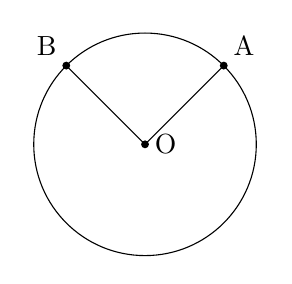
\begin{tikzpicture}[bar width=0.4]
            \coordinate (A) at (1,1);
            \coordinate (B) at (-1,1);
            \coordinate (O) at (0,0);
            \node at (A) [above right] {A};
            \node at (B) [above left] {B};
            \node at (O) [right] {O};
            \fill (A) circle (0.05);
            \fill (B) circle (0.05);
            \fill (O) circle (0.05);
            \coordinate [draw, name path=o, circle through=(A)] (o) at (O);
            \draw (A) -- (O);
            \draw (B) -- (O);
        \end{tikzpicture}
        \caption{圆、弧}
    \end{minipage}
\end{figure}

在平面几何中,还有一种常见的图形是圆. 作一个圆需要用到圆规. 到一个点 $A$ 距离相等的所有点构成了一个圆,这个距离称作这个圆的半径. 

图 5 中,$A,B$ 两点将圆分为了两部分,较小的一部分为劣弧,记作 $\wideparen{AB}$. 较大的一部分称为优弧,记作 $\wideparen{AmB}$. 我们通常
讨论的是劣弧.

以 $O$ 为圆心、$r$ 为半径的圆通常可以记为 $\odot O$ 或 $\odot (O,r)$.

\subsection{全等三角形}

\end{document}
